\chapter{State of the Art} \label{chap:State of the Art}
% introduction

\section{Implementation of Reactive Systems}
	\subsection{Reactive Programming}
	%"Reactive programming provides dedicated language abstractions for reactive software. Reactive programming relieves developers from manually updating outputs when the inputs of a computation change, it overcomes a number of well-know issues of the Observer design pattern, and it makes programs more comprehensible." [github, rxScala guido] Its also declarative instead of imperative.
	% reactive programming is in general not asynchroneous but it can be used in async context.? (waqas says something different for RXjs)
	% observables, difference to Observer design pattern:
		% observables in a reactive system return/provide multiple values (a stream) instead of just the current state.
		% "Observables provide abstractions over a stream of events. Promises are synchronous executables with a single return value, whereas observables are asynchronous executables that return multiple values over time." [pradeep]
		%"The data produced by the producer is stored in observable which the consumer consumes."[Pradeep]
	% observables are also called signals[wikipedia] = values that vary over continuous time -> or in RxJs Observables, Bacon Properties
	% events = events which have occurrences at discrete points in time -> RxJs Subject, Bacon EventStream
	% "observables" are functions that tie an observer to a producer. A producer creates values over time. An observer reacts to the values of a producer and notifies all subscribers (in a push based system).
	%operators: "Each operator outputs an another observable without modifying the original data streams." [Pradeep]
	% push and pull based: 
		%"Push-based systems take events and push them through a signal network to achieve a result. Pull-based systems wait until the result is demanded, and work backwards through the network to retrieve the value demanded." https://en.wikipedia.org/wiki/Functional_reactive_programming
	% cold and hot observables https://medium.com/@benlesh/hot-vs-cold-observables-f8094ed53339
			% -> author: "RxJS 5+ Lead, Software Engineer at Google, RxWorkshop.com. Own view, not the companies"
		% cold: the subscribe call creates the producer - one producer (e.g. a websocket raising events) is created for each call to subscribe, it gets destroied if the observer unsubscribes -> unicast
		% hot: all calls to subscribe (usally) share one producer - multicast
		% Rx Subjects - functions as both observer and observable, multicast but will terminate if the last subscriber is unsubscribed, can not be reused after termination or if in error state. "It multicasts. All observers passed to it via `subscribe()` are added to an internal observers list."
			% "Armed with our Rx Subject above, we can use a bit of functional programming to make any “cold” observable “hot”:
			%function makeHot(cold) {const subject = new Subject();cold.subscribe(subject); return new Observable((observer) => subject.subscribe(observer));}
			%Our new `makeHot` method will take any cold observable and make it hot by creating a subject that is shared by the resulting observable."
			% in RxJs that is e.g. publish or share
	
	\subsection{RxJs and BaconJs}
	% Though there are other Javascript implementations of the reactive design pattern like https://github.com/stoeffel/awesome-frp-js,
	% kefir, cyclejs
	% this thesis focuses on RxJs and BaconJs, because these are the one the extension currently supports.
	
	%RXjs
	%var button = document.querySelector('button');
	%Rx.Observable.fromEvent(button, 'click')
	%.throttleTime(1000)
	%.scan(count => count + 1, 0)
	%.subscribe(count => console.log(`Clicked ${count} times`));
	% The essential concepts in RxJS which solve async event management are:
	%Observable: represents the idea of an invokable collection of future values or events.
	%Observer: is a collection of callbacks that knows how to listen to values delivered by the Observable.
	%Subscription: represents the execution of an Observable, is primarily useful for cancelling the execution.
	%Operators: are pure functions that enable a functional programming style of dealing with collections with operations like map, filter, concat, flatMap, etc.
	%Subject: is the equivalent to an EventEmitter, and the only way of multicasting a value or event to multiple Observers.
	%Schedulers: are centralized dispatchers to control concurrency, allowing us to coordinate when computation happens on e.g. setTimeout or requestAnimationFrame or others.
	%"The subscribers are not locked in a synchronous request and there can be an infinite sequence of next emissions from the observables to the observer." [Pradeep] although subscribing is in general a synchroneous operation.
	%"completed and error functions	being defined at the observer, which are invoked by the observable on respective events. This lets the observer know that an observable has exhausted sending values, or an error has occurred	when performing an operation on the observable." [Pradeep]
	%"Subjects can be both observable and an observer[37]. It is a special type of observable which	allows values to be multicasted to many observers" [Pradeep]
	%"Unsubscribing is an optional feature in RxJS as RxJS handles this by default but it makes sense to unsubscribe manually by a user if the source observable is emitting the values continuously and the user does not need values after a specific point of time." [Pradeep]
	%"With the support of RxJS, we can convert multiple values, arrays, events into observables."[Pradeep]
	
	
	%Baconjs: 
	%Generally, this is how you implement an app with Bacon.js. Capture input into EventStreams and Properties - Transform and compose signals into ones that describe your domain. - Assign side-effects to signals.
	%EventStreams (distinct events) and Properties (values that change over time). 
	%$("#username input").asEventStream("keyup").map(function(event) { return $(event.target).val() }).toProperty("")
	% "In Bacon, these are two flavors of Observables. EventStreams and Property are two basic concepts	of Bacon.js that are basically known as events and behaviours in the literature of FRP." [waqas]

	\subsection{Debugging Reactive Code}
	% due to reactive programming being declarative ... [github, guido rxScala]
	% short-comings of standard debuggers with reactive systems:
		% - stepping through reactive libarary code to track down bugs
		% - unconditional breakpoints in lambda functions will trigger to often to be useful 
		% - non-linear code execution makes step by step debugging hard -> "step over" is rarely useful and "step into" needs to be used multiple times for chained functions to iterate to the desired part, because "step over" will skip the whole line [verify with VS, IntelliJ, Webstorm, Chrome debugger].
		%- "lack of abstractions" and "mismatch in the mental model" [paper guido1]
		% - "Missing dependencies are hard to detect with traditional debuggers." [paper guido1 4.1]
	% - unit tests and do-debugging for Rx: https://msdn.microsoft.com/en-us/library/hh242967(v=vs.103).aspx to reduce the effort of adding do-statements each time a bug is tracked down, the developer can add logging functionality and use that in the do statement. https://shiny.rstudio.com/articles/debugging.html #"The Reactive log" where a visualization is later used on the log to create a simple dependency graph containing code pieces as nodes.
	% other systems that do
	% - Reactive Inspector for scala https://guidosalva.github.io/reactive-inspector/ is an extension of Scala IDE for Eclipse. Reactive Inspector is a project started and maintained by Guido Salvaneschi at the Software Technology Group - Technical University of Darmstadt, Germany and many people have contributed.
		% - Many features and the basic concepts that are implemented in CRI originate from RxScala Reactive Inspector. Dependency graph in the so called Reactive Tree, Tree History, History Queries, Reactive Breakpoints, Node search/dependencies/dependents. They are described in details in [Chapter: Previous CRI]
		% -"Tree Outline: Tree Outline In a large dependency graph it is sometimes hard to navigate the reactive tree. This view shows you at a glance where you are in the graph and helps you jump quickly to a different area of the graph."
	% - reference to rxfiddle in later section

\section{Previous and Related Work}
	\subsection{The Chrome Reactive Inspector}
		\subsubsection{Master Thesis by Waqas Abbas}
		% main focus of the thesis
			% - proof of concept
			% - how to intercept calls to reactive framework
			% - how to retrieve additional details for each node like the variable name via instrumentation of the source code to give context to observables shown in the dependency graph
		% implemented result of the thesis in short
			% - reactive breakpoints
			% - history queries
			% - Bacon support and partly support for Rx
			% - dependency graph, nodes, edges, zoom, highlighting of current node
			% - instrumentation, dynamically reloading of the page to intercept the javascripts for instrumentation
			% - first batch of test applications
			% -> focus on new implementation and prototypes of features and less on maintainability and reliability.
			% -> proof of concept
		
		\subsubsection{Master Thesis by Pradeep Baradur}
		% main focus of the thesis:
			% support for all RxJS operations and RxJS Subjects -> hard to implement, because there is no uniform way like the Bacon.spy method. For details on the general approach see [ref to pradeep thesis]. For source code see "rx-interception.js"
		% new features introduced:
			% - support for all operations and Subjects in RxJs
			% - loading of some CRI content scripts only when the CRI panel is opened. Istrumentation only when CRI panel is opened.
			% - find dependencys, dependents
			% - added many test applications
			% - improved reliability
			% - less focus on maintainability but move the project further to being usable in a production environment by adding framework feature support.
			% - rearranged UI, changed many styles to defaullt jquery-ui layout.
		
		\subsubsection{Merging previous efforts}
		%- took chrome-reactive-inspector 2 as base and merge all later developed features into it, piece by piece. manually copied changes by Pradeep from Waqas's repository. Hard to detect, changed to match other variable names before committing.
		% - uncompatible git histories - solvable but not much use since the files had separated so much in text character changes, though not so much in logic -> renames and splitting of files
		% - access to many global variables made tracking down dependencies of components hard with mixed contexts - some files with the window object corresponding to contentscripts in the same directory as files with a window object corresponding to the extensions window.
		%TODO: change tone to always present problems as general difficulties instead of shortcomings
		% - merged additional features of Abbas with framework support from Pradeep
		
		\subsubsection{"Special Curicumstances"}
		% demo version of jalangi
		% instrumenting files via scanning the html for script tags
		% -> will not work for module loaders like require.js or ecma6
		% -> will not work with bundled javascript code - but since in development there should be a non bundled version available not 
		% a big problem in javascript. But for Typescript since the extension does not support it and when compiling there may already be bundling in place. (#add some text from future here#)
		
		% Shared context through "new Function" that breaks the separation enforced by chrome. To increase consistency and prevent different execution contexts the previous eval was replaced with "new Function" but this does not reduce the security risk.There are other options to execute scripts from a chrome extension but since some of the extension scripts need to share the Rx or Bacon object with the inspected pages javascript files there is no other way. ofcorse that breaks the normal isloated world and intodruces a new set of problems like conflicting names. The security risk involved in executing a foreign script in a "trusted" extension context could be reduced if a sandbox was used as described in https://developer.chrome.com/extensions/sandboxingEval. Then all the inspected pages content scripts and some special recording scripts could be executed in that sandbox and transmitt the recorded nodes back via message passing.
		% - Dangers of using eval -> execution in current context. if called from other function, "this" might change. Function() for global with window passed to execute in original context.
		%- Note that  files that are not selected for instrumentation will still generate nodes in the graph, because the Rx and Bacon frameworks will still record interactions, just the information provided by instrumentation is missing.
		%- The Bacon and Rx scripts are prevented from loading so the extensions own files can be used. This is accomplished by filtering all referenced js files in the inspected page for any Bacon or Rx library files and excluding them from the loading process. They need to match version exactly though. This is necessary to guarantee that both work with the same Rx/Bacon object.
	

	\subsection{RxFiddle}
	% RxFiddle is the main competitor with CRI since it is the only other tool (that we are aware of) that tackels debugging for reactive javascript systems. Currently the only reactive framework that is supported is RxJs.
	% features of RxFiddle
	% limitations: 'one of the limitations of RxFiddle is ... which we tackeld in this work.
		% - requires more setup to use with web sites that have DOM logic and applications with more than one Javascript files, although it is possible according to the author [ref rxfiddle attached].
		% - the variable names in the source code are not displayed in the ui. RxFiddle instruments RxJs to collect its data, not the source code itself like CRI.
		% - fast updating observables like "interval" since each value update creates a new marble for the observable, the view becomes encoumbered fast with this type of observables. As of this moment CRI also generates one or more steps for each update (if the node is not explicitly excluded), but it is easier to examine the value of a node in the first or last few steps (jump to the step and use the next/previous button). CRI can also query the result which provide means to cope with large dependency graphs or histories. In RxFiddle the limitating factor for the fine grained stepping is the available space and resulting overplotting of the value-marbles since the examination is implemented via tooltips on mouseover. For performance comparison see [Evalutation chapter section Performance Improvements].
		% - like the author explained in "https://github.com/hermanbanken/RxFiddle/issues/6" the web app can not work with large applications properly. The displaying of large applications in one graph is hard for both tools [reference to Contributions chapters], but RxFiddle needs more spaces for a single reactive operator than CRI. A large dependency graph with descriptive nodes is easier to examine than a large marble diagram that only shows information on nodes in tooltips except in the details view of a currently selected node so finding the desired node/operation is not as easy. RxFiddle also has performacne issue while rendering huge diagrams according to the author. RxFiddle would porbably need another view to appropiately cope with such large applications to help the user navigate and give an overview, although for mid-sized applications the graph on the left side where a user can choose which operation to examine can serve this purpose - As mentioned earlier RxFiddle does not porvide variable names which may lead to confusion of nodes if similar observables are in the same application.
		% As of now, CRI does not support multiple variables having the same name. The author describes some other options like priority ranking in the issue [ref].
		% - as mentioned erlier RxFiddle onyl supports RxJs while CRI also supports Bacon.js
	% - The author plans to support multiple collectors in the future for web applications, RxScala, RxJava, RxSwift and/or RxNet (source: "https://rxfiddle.net/tutorials.html#attached") which would provide the necessary data collection on one of these platforms and transmit this data to the RxFiddle tool/web-application to be able to use the same debugging environment (RxFiddle) with any of these platforms.



% end of state of the art chapter
%----------------------------------------------------------------------------
%latex sample code:



\begin{figure}[!h]
	\centering
	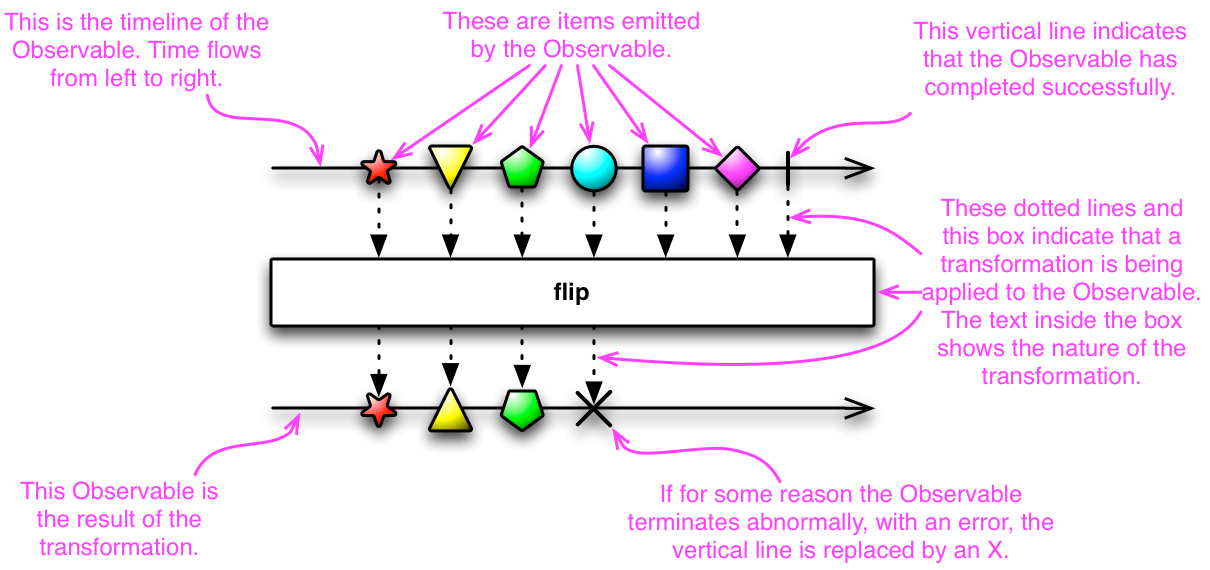
\includegraphics[scale=0.5,trim=0 0 0 0]{gfx/rxjs-reactive-pattern2.png}
	\caption{Reactive pattern \protect\cite{ReactiveXobservable}}
	\label{fig:rxjs-reactive-pattern}
\end{figure}

\textbf{Observable and Observer}\\
Placeholder

\textbf{Operators}
\label{subsec:Operators}\\

\textbf{RxJS Code Structure}\\
Placeholder
\begin{lstlisting}[language=JavaScript, caption=RxJS Simple Example, label={lst:RxJS_Simple_Example}]
// 1. Srouce Observable Creation
var sourceObservable = Rx.Observable.interval(1000);
// 2. Transformation by applying different operators
var transformedObservable = sourceObservable.map(function(x) {
		return x * 10;
	})
	.filter(function(x) {
		return x !== 20
	})
// OUTPUT
Next: 0
Next: 10
Next: 30
Next: 40
Next: 50
Completed
\end{lstlisting}

\subsection{Bacon.js}

\textbf{EventStream and Property}\\
Placeholder

